\documentclass[11pt,a4paper]{article}

% ------------------------------------------------------------------ %
% Packages (chosen to compile cleanly with tectonic / XeTeX)          %
% ------------------------------------------------------------------ %
\usepackage[margin=1in]{geometry}
\usepackage{graphicx}
\usepackage{booktabs}
\usepackage{longtable}
\usepackage{array}
\usepackage[table]{xcolor}
\usepackage{enumitem}
\usepackage{tikz}
\usetikzlibrary{positioning,arrows.meta,shapes.geometric,fit,backgrounds,calc}
\usepackage{caption}
\usepackage{subcaption}
\usepackage{amsmath}
\usepackage{float}
\usepackage{listings}
\usepackage{underscore} % lets bare _ print in text/tables (many snake_case tokens)
\usepackage[hidelinks]{hyperref}

\graphicspath{{figures/}}

% ------------------------------------------------------------------ %
% Status colours + macros                                             %
% ------------------------------------------------------------------ %
\definecolor{cok}{HTML}{1B7F3B}     % green   - complete / verified
\definecolor{cpart}{HTML}{B26B00}   % orange  - partial / pending
\definecolor{cmiss}{HTML}{B00020}   % red     - missing / blocked
\definecolor{cnv}{HTML}{5A5A5A}     % gray    - not verified
\definecolor{hdr}{HTML}{123A5E}

\newcommand{\stC}{\textcolor{cok}{\textbf{COMPLETE}}}
\newcommand{\stV}{\textcolor{cok}{\textbf{VERIFIED}}}
\newcommand{\stP}{\textcolor{cpart}{\textbf{PARTIAL}}}
\newcommand{\stPend}{\textcolor{cpart}{\textbf{PENDING}}}
\newcommand{\stM}{\textcolor{cmiss}{\textbf{MISSING}}}
\newcommand{\stB}{\textcolor{cmiss}{\textbf{BLOCKED}}}
\newcommand{\stNV}{\textcolor{cnv}{\textbf{NOT VERIFIED}}}
\newcommand{\yes}{\textcolor{cok}{yes}}
\newcommand{\no}{\textcolor{cmiss}{no}}
\newcommand{\code}[1]{\texttt{\small #1}}

\lstset{
  basicstyle=\ttfamily\footnotesize,
  breaklines=true,
  frame=single,
  columns=fullflexible,
  keepspaces=true,
  showstringspaces=false,
  xleftmargin=0.5em
}

% TikZ node styles
\tikzset{
  box/.style={rectangle, rounded corners=2pt, draw=hdr, fill=blue!5, thick,
              text width=2.7cm, align=center, minimum height=0.9cm, font=\small},
  src/.style={rectangle, rounded corners=2pt, draw=cok, fill=green!6, thick,
              text width=2.6cm, align=center, minimum height=0.8cm, font=\small},
  warn/.style={rectangle, rounded corners=2pt, draw=cpart, fill=orange!8, thick,
               text width=2.6cm, align=center, minimum height=0.8cm, font=\small},
  flow/.style={-{Stealth[length=2.2mm]}, thick, draw=hdr}
}

\hypersetup{
  pdftitle={SuryaGrid AI: Current Implementation Status and Real-Data Roadmap},
  pdfauthor={Lekhan HR / SuryaGrid Project}
}

% ------------------------------------------------------------------ %
\begin{document}

\begin{titlepage}
\centering
\vspace*{2.2cm}
{\Huge\bfseries SuryaGrid AI\par}
\vspace{0.5cm}
{\LARGE Current Implementation Status and Real-Data Roadmap\par}
\vspace{0.8cm}
{\large Bengaluru / Karnataka / India Solar-Grid Forecasting\\ and DSM Multi-Agent Platform\par}
\vspace{2cm}
{\large\itshape Technical Implementation Report\par}
\vspace{1.5cm}
\begin{tabular}{rl}
\textbf{Author:} & Lekhan HR / SuryaGrid Project\\[4pt]
\textbf{Date:} & 6 July 2026\\[4pt]
\textbf{Scope:} & Verified repository state only\\[4pt]
\textbf{Repositories:} & DBIT-Banglore/SuryaGrid, lekhanpro/SuryaGrid\\
\end{tabular}
\vfill
{\footnotesize All claims in this report are grounded in inspected files, generated
artifacts, model cards, and command outputs captured on the dates shown. Items that
could not be verified are marked \stNV, \stPend, or \stM\ rather than asserted.\par}
\end{titlepage}

\tableofcontents
\newpage

% ================================================================== %
\section*{Abstract}
\addcontentsline{toc}{section}{Abstract}
SuryaGrid AI is a multi-agent solar-grid forecasting and Deviation Settlement Mechanism
(DSM) support platform focused on Bengaluru / Karnataka / India. This report documents
the \emph{verified} state of the repository as of 6 July 2026. The backend (FastAPI)
exposes 54 registered endpoints across 15 routers and passes its full test suite
(93 tests). A real-data ML pipeline has been executed: an hourly Bengaluru
weather/solar history of 26{,}304 rows (2022--2024) was ingested from the Open-Meteo
historical archive and cross-checked against NASA POWER (daily GHI Pearson
$r=0.87$); 344 substations were ingested from OpenStreetMap; and India national hourly
demand (11{,}664 rows) was downloaded from Kaggle. Four models were trained and carry
model cards: a solar irradiance forecaster ($R^2=0.956$), a cloud/irradiance-drop-risk
classifier ($F_1=0.67$, AUC $=0.90$), and a DSM deviation-breach classifier
($F_1=0.79$); a load forecaster trained on India-national data ($R^2=0.88$) is
explicitly marked \emph{not} production-ready due to high geographic domain shift. The
reinforcement-learning policy is intentionally \emph{not} trained (no real local load,
no official tariff reward). The frontend (Next.js 14) builds successfully (14 static
routes). Docker configuration exists but was \emph{not} executed in this environment
(the \code{docker compose} subcommand is unavailable and the daemon is unreachable).
Local PV generation data, metered Karnataka load, official parsed tariff/DSM rupee
rates, and substation capacity are \emph{not} present and are tracked honestly as
pending. The platform is therefore best characterised as an architecturally complete,
partially data-complete prototype; it is not full production-ready.

% ================================================================== %
\section{Introduction}
\subsection{Project goal}
SuryaGrid AI turns real meteorological data into a solar generation/irradiance forecast
(physics via pvlib and ML via scikit-learn), compares forecast injection against a
schedule, and classifies DSM deviation risk, with every reported value traceable to a
source. It is organised as a set of deterministic Python agents behind a FastAPI service
and a Next.js dashboard.

\subsection{Why the Bengaluru / Karnataka / India context matters}
Solar output, grid tariffs, deviation-settlement rules, load shape, and substation
topology are all region-specific. A forecaster or DSM engine calibrated on foreign data
(for example the Hawaii HI-SEAS Kaggle set) does not transfer faithfully to Bengaluru.
The project therefore prioritises, in order: Bengaluru-specific, Karnataka-specific,
South-India, India-wide, coordinate-based global APIs at Bengaluru's coordinates, and
only then non-local data as a labelled baseline.

\subsection{Data honesty taxonomy}
The codebase distinguishes real data (measured/observed), estimated data (derived from
real inputs via a documented formula), synthetic-augmented data (labelled, never used as
production truth in real mode), and demo data. Two complementary source-tracking systems
exist in the repo: a Phase~1.5 registry (\code{app/data\_sources/source\_registry.py})
and a Phase~1.7 provenance-label system (\code{app/ml/provenance.py}).

% ================================================================== %
\section{Scope of This Report}
This report documents the current repository state only. Every status is derived from one
or more of: directory listings, file contents, generated artifacts (parquet, pkl, JSON
model cards, build/training manifests), the FastAPI route table introspected from the
running application object, the test runner, the linter, and the frontend build. Where a
capability is designed but not executed or not present, it is labelled \stPend, \stNV, or
\stM. No metrics, endpoints, or datasets are invented; numeric metrics are quoted verbatim
from the model cards and manifests.

% ================================================================== %
\section{Repository Overview}
The repository contains a Python/FastAPI backend, a Next.js frontend, an extensive
\code{docs/} tree, generated ML data and models, and Docker configuration.
Table~\ref{tab:components} summarises the major components and their verified status.

\begin{table}[H]
\centering
\caption{Component status (Table 1).}
\label{tab:components}
\footnotesize
\begin{tabular}{@{}p{2.6cm}p{3.1cm}p{4.2cm}l l@{}}
\toprule
\textbf{Component} & \textbf{Path} & \textbf{Purpose} & \textbf{Status} & \textbf{Evidence}\\
\midrule
Backend API & \code{backend/app} & FastAPI service, 15 routers & \stC & 54 routes; 93 tests\\
Agents & \code{backend/app/agents} & 16 agent modules & \stC & files + workflows doc\\
ML pipeline & \code{backend/app/ml} & build + train + inference & \stP & artifacts generated\\
Data sources & \code{backend/app/data\_sources} & providers + registry & \stP & OSM/Open-Meteo wired\\
DSM engine & \code{backend/app/dsm} & rule profiles + classifier & \stP & framework only (no INR)\\
Frontend & \code{frontend/} & Next.js 14 dashboard & \stC & build passes, 14 routes\\
ML datasets & \code{backend/data/ml} & 8 parquet + manifests & \stP & files present\\
Trained models & \code{backend/models/trained} & 4 pkl + rules engine & \stP & 4/5 trained\\
Model cards & \code{backend/models/metadata} & 5 cards + run manifest & \stC & all present\\
Tests & \code{backend/tests} & pytest suite & \stV & 93 passed\\
Docker & \code{docker-compose.yml}, Dockerfiles & 4-service stack & \stNV & not run here\\
Docs & \code{docs/} & 24 markdown files & \stC & inventory in Sec.~\ref{sec:docs}\\
\bottomrule
\end{tabular}
\end{table}

% ================================================================== %
\section{System Architecture}
Figure~\ref{fig:arch} shows the high-level pipeline: real data sources are ingested and
validated, materialised into ML datasets, used to train models, wrapped by agents,
sequenced by an orchestrator, exposed through FastAPI, and rendered by the frontend.

\begin{figure}[H]
\centering
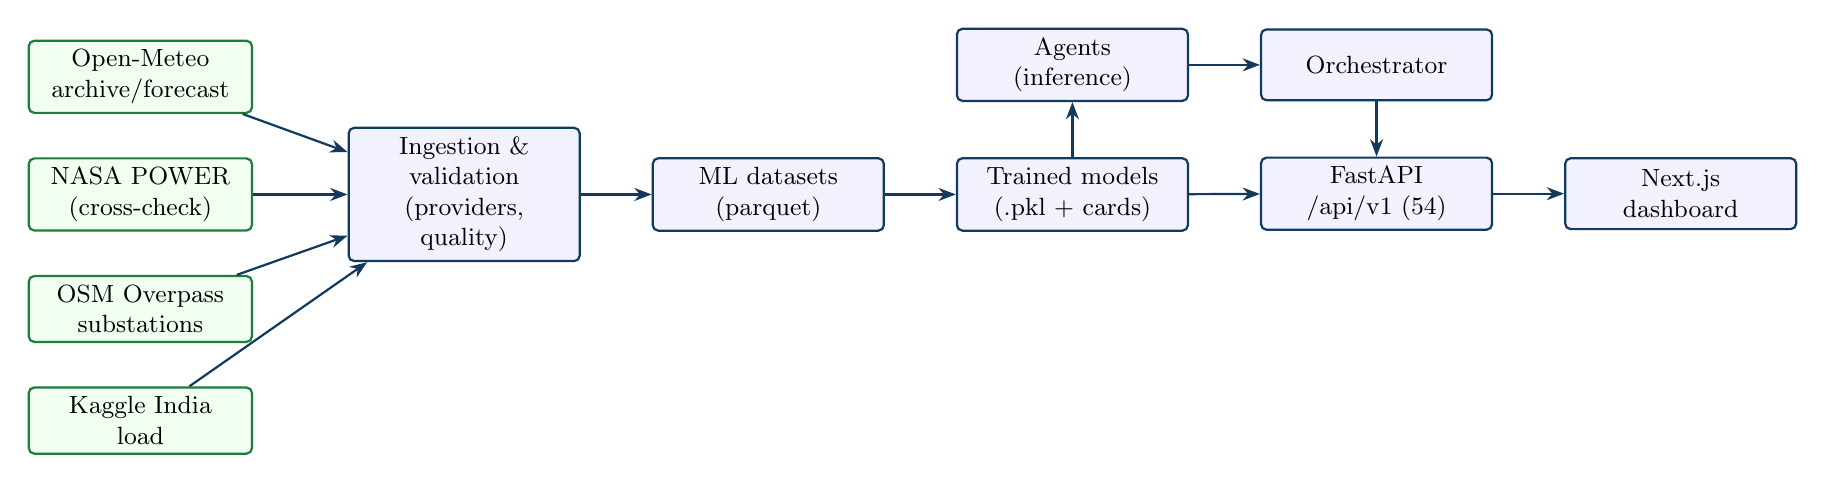
\begin{tikzpicture}[node distance=0.55cm and 0.9cm]
\node[src] (om) {Open-Meteo\\archive/forecast};
\node[src, below=of om] (nasa) {NASA POWER\\(cross-check)};
\node[src, below=of nasa] (osm) {OSM Overpass\\substations};
\node[src, below=of osm] (kag) {Kaggle India\\load};
\node[box, right=1.2cm of nasa] (ing) {Ingestion \&\\validation\\(providers, quality)};
\node[box, right=of ing] (ds) {ML datasets\\(parquet)};
\node[box, right=of ds] (tr) {Trained models\\(.pkl + cards)};
\node[box, above=0.7cm of tr] (ag) {Agents\\(inference)};
\node[box, right=of ag] (orc) {Orchestrator};
\node[box, below=0.7cm of orc] (api) {FastAPI\\/api/v1 (54)};
\node[box, right=of api] (fe) {Next.js\\dashboard};

\draw[flow] (om) -- (ing); \draw[flow] (nasa) -- (ing);
\draw[flow] (osm) -- (ing); \draw[flow] (kag) -- (ing);
\draw[flow] (ing) -- (ds); \draw[flow] (ds) -- (tr);
\draw[flow] (tr) -- (ag); \draw[flow] (ag) -- (orc);
\draw[flow] (orc) -- (api); \draw[flow] (tr) -- (api);
\draw[flow] (api) -- (fe);
\end{tikzpicture}
\caption{High-level SuryaGrid architecture (Figure 1). Green = real external sources;
blue = internal stages. NASA POWER is currently wired only as a build-time cross-check,
not as a live weather provider (Sec.~\ref{sec:datasources}).}
\label{fig:arch}
\end{figure}

\noindent\textbf{Backend.} Python 3.11/3.12, FastAPI, SQLAlchemy (SQLite default;
PostgreSQL via Docker), Redis cache (optional), pvlib + scikit-learn for the numeric
path. \textbf{Frontend.} Next.js 14 / React / Tailwind, static-export capable
(\code{frontend/out/} present). \textbf{Storage/artifacts.} ML datasets in
\code{backend/data/ml/}, models in \code{backend/models/trained/}, cards in
\code{backend/models/metadata/}.

% ================================================================== %
\section{Data Sources and Real-Data Status}
\label{sec:datasources}
Table~\ref{tab:sources} classifies every source found in the code, the Phase~1.5 source
registry, or the Phase~1.7 build manifest. A source is only listed if it appears in the
repository.

\begin{footnotesize}
\begin{longtable}{@{}p{2.7cm}p{1.5cm}p{2.0cm}p{3.0cm}p{2.2cm}p{2.4cm}@{}}
\caption{Data source status (Table 2).}\label{tab:sources}\\
\toprule
\textbf{Source} & \textbf{Type} & \textbf{Geography} & \textbf{Implementation status} & \textbf{Evidence} & \textbf{Limitation}\\
\midrule
\endfirsthead
\multicolumn{6}{c}{\tablename\ \thetable{} -- continued}\\
\toprule
\textbf{Source} & \textbf{Type} & \textbf{Geography} & \textbf{Implementation status} & \textbf{Evidence} & \textbf{Limitation}\\
\midrule
\endhead
\bottomrule
\endfoot
Open-Meteo archive & weather & coordinate (Bengaluru) & \stV\ wired \& used & 26{,}304 rows; manifest & reanalysis, not on-site\\
Open-Meteo forecast & weather & coordinate & \stV\ wired (live provider) & \code{source\_registry.py}; tests & fair-use limits\\
NASA POWER & weather & coordinate (Bengaluru) & API reachable; used as cross-check; live-provider integration \stPend & manifest $r=0.87$; registry ``not yet wired'' & not a runtime provider yet\\
Kaggle India load & dataset & India (national) & \stV\ downloaded \& used & 11{,}664 rows parquet & non-local; domain-shift high\\
Kaggle HI-SEAS & dataset & Hawaii (non-local) & registered; \textbf{not} used by trained models & \code{source\_registry.py} & PRETRAINING\_ONLY only\\
OSM / Overpass & substation & Bengaluru/Karnataka & \stV\ wired \& used & 344 rows parquet & voltage 41\%; capacity 0\%\\
KERC / BESCOM tariff & dsm\_rule & Karnataka & framework only; rates \stPend & registry; verification doc & no parsed INR rates\\
CERC DSM 2024 & dsm\_rule & India & framework only; rates \stPend & registry; verification doc & market-linked; litigated\\
CEA emission/load & dataset & India & referenced in research doc; \textbf{not} wired & research doc only & no adapter/code\\
KPTCL-SLDC / Grid India & load & Karnataka/India & documented; \textbf{not} wired & research doc & portal/PDF, no API\\
Solcast & weather & coordinate & reserved slot; \textbf{not} wired & registry & requires API key\\
Synthetic weather & synthetic & n/a & present as labelled fallback; blocked in real mode & \code{synthetic\_weather\_provider.py} & demo only\\
\end{longtable}
\end{footnotesize}

\noindent Classification labels observed in the Phase~1.7 provenance system and cards:
\code{REAL\_COORDINATE\_BASED} (weather/solar), \code{REAL\_BENGALURU} /
\code{REAL\_KARNATAKA} (substations), \code{REAL\_INDIA} (load),
\code{ESTIMATED\_FROM\_REAL} (grid geometry, clear-sky), \code{NEEDS\_OFFICIAL\_SOURCE}
(tariff/DSM rupees), \code{NOT\_AVAILABLE} (RL environment, local PV).

% ================================================================== %
\section{Data Mode and Source Tracking}
Table~\ref{tab:datamode} records the source-tracking and data-mode mechanisms actually
present.

\begin{table}[H]
\centering
\caption{Data-mode and source-tracking mechanisms (Table 3a).}
\label{tab:datamode}
\footnotesize
\begin{tabular}{@{}p{3.2cm}c p{4.0cm}p{3.6cm}@{}}
\toprule
\textbf{Mechanism} & \textbf{Implemented?} & \textbf{File / behavior} & \textbf{Missing work}\\
\midrule
\code{APP\_DATA\_MODE} & \yes & \code{config.py} default \code{real} & UI toggle not exposed\\
Real-mode synthetic block & \yes & \code{provenance.assert\_real\_mode\_allows} raises \code{SyntheticFallbackError} & enforced in ML scripts; not globally in every legacy route\\
Phase 1.5 source registry & \yes & \code{source\_registry.py} (8 records) + \code{/sources} API & DB-backed re-verification\\
Phase 1.7 provenance labels & \yes & \code{provenance.py}; model cards carry \code{source\_status}, \code{data\_mode} & unify with 1.5 registry\\
Model cards & \yes & 5 cards, required-field validation & --\\
\bottomrule
\end{tabular}
\end{table}

\noindent The real-mode guard is exercised by the test suite (a dedicated test asserts
that synthetic/demo labels raise in \code{real} mode). Enforcement is strongest inside the
ML build/train scripts; older Phase~1 prediction routes retain a labelled synthetic
weather fallback and are not governed by the same hard guard.

% ================================================================== %
\section{ML Dataset Creation}
All datasets below were generated by
\code{python -m app.ml.build\_ml\_datasets --region bengaluru --data-mode real} and are
recorded in \code{backend/data/ml/dataset\_build\_manifest.json}. Row counts are quoted
from that manifest and from the files on disk.

\begin{footnotesize}
\begin{longtable}{@{}p{4.0cm}c p{2.3cm}p{2.6cm}p{1.4cm}c@{}}
\caption{ML dataset status (Table 3).}\label{tab:mldata}\\
\toprule
\textbf{File (backend/data/ml/)} & \textbf{Exists} & \textbf{Geography} & \textbf{Source / label} & \textbf{Rows} & \textbf{Status}\\
\midrule
\endfirsthead
\toprule
\textbf{File} & \textbf{Exists} & \textbf{Geography} & \textbf{Source / label} & \textbf{Rows} & \textbf{Status}\\
\midrule
\endhead
\bottomrule
\endfoot
bengaluru\_weather\_solar\_history.parquet & \yes & Bengaluru coord & Open-Meteo+NASA / REAL\_COORDINATE\_BASED & 26{,}304 & \stV\\
bengaluru\_substations\_cleaned.parquet & \yes & Bengaluru/Karnataka & OSM / REAL\_BENGALURU & 344 & \stV\\
bengaluru\_grid\_features.parquet & \yes & Bengaluru & geometry / ESTIMATED\_FROM\_REAL & 344 & \stV\\
solar\_agent\_training.parquet & \yes & Bengaluru coord & REAL\_COORDINATE\_BASED & 26{,}304 & \stV\\
cloud\_agent\_training.parquet & \yes & Bengaluru coord & REAL\_COORDINATE\_BASED & 12{,}041 & \stV\\
dsm\_agent\_training.parquet & \yes & Bengaluru coord & REAL\_COORDINATE\_BASED & 12{,}031 & \stV\\
karnataka\_or\_india\_load\_history.parquet & \yes & India national & Kaggle / REAL\_INDIA & 11{,}664 & \stP\ (non-local)\\
load\_agent\_training.parquet & \yes & India national & REAL\_INDIA & 11{,}496 & \stP\ (non-local)\\
rl\_environment\_dataset.parquet & \no & --- & NOT\_AVAILABLE & 0 & \stM\\
\end{longtable}
\end{footnotesize}

\noindent Provenance highlights recorded in the manifest: the weather history spans
2022-01-01 to 2024-12-31 with a peak GHI of 1044 W/m2; the Open-Meteo vs NASA POWER daily
GHI agreement is Pearson $r=0.8728$ over 1{,}096 days; substations have voltage on 41\%
of records and capacity on 0\% (kept null, never invented). Each dataset row carries
\code{source\_name}, \code{data\_geography}, \code{ingestion\_time}, and a
\code{quality\_score} (weather mean 0.994).

% ================================================================== %
\section{Model Training and Model Artifacts}
Metrics are quoted verbatim from the model cards in \code{backend/models/metadata/}.
Splits are chronological 80/20.

\begin{footnotesize}
\begin{longtable}{@{}p{2.4cm}p{2.6cm}p{3.3cm}c p{2.4cm}@{}}
\caption{Model artifact status (Table 4).}\label{tab:models}\\
\toprule
\textbf{Model} & \textbf{File / card} & \textbf{Metrics (held-out)} & \textbf{Prod?} & \textbf{Reason / limit}\\
\midrule
\endfirsthead
\toprule
\textbf{Model} & \textbf{File / card} & \textbf{Metrics} & \textbf{Prod?} & \textbf{Reason / limit}\\
\midrule
\endhead
\bottomrule
\endfoot
Solar irradiance & solar\_forecast\_model.pkl / card & $R^2$=0.9563, RMSE=57.51, MAE=29.12 W/m2 & \yes & GHI only; PV not predicted\\
Cloud drop-risk & cloud\_risk\_classifier.pkl / card & $F_1$=0.6707, AUC=0.9001, acc=0.866 & \yes & irradiance drop, not PV drop\\
DSM breach & dsm\_classifier.pkl + dsm\_rules\_engine.json / card & $F_1$=0.7905, AUC=0.7489, acc=0.712 & \yes & no INR; +/-15\% modelling band\\
Load forecast & load\_forecast\_model.pkl / card & $R^2$=0.883, RMSE=6259.5 MW & \no & INSUFFICIENT\_LOCAL\_LOAD\_DATA; domain shift HIGH\\
Weather correction & --- & --- & \no & not implemented (no separate model)\\
RL policy & rl\_policy.zip \textbf{absent} / card present & none (not trained) & \no & INSUFFICIENT\_REAL\_ENVIRONMENT\_DATA\\
\bottomrule
\end{longtable}
\end{footnotesize}

\noindent The solar card records train/test = 21{,}043/5{,}261; cloud = 9{,}632/2{,}409;
DSM = 9{,}624/2{,}407; load = 9{,}196/2{,}300. All cards report
\code{uses\_synthetic\_data=false}, \code{synthetic\_percentage=0}, and
\code{data\_mode=real}. The DSM card and rules engine assert
\code{emits\_rupee\_values=false}.

% ================================================================== %
\section{Agent Design and Working}
Per \code{docs/AGENT\_WORKFLOWS.md}, agents are deterministic Python coordinators (no LLM
in the numeric path). Sixteen agent modules exist under \code{backend/app/agents/}. The
Phase~1.7 ML inference layer (\code{app/ml/agent\_models.py}) additionally serves the
trained models behind the \code{/api/v1/agents/*} endpoints. Table~\ref{tab:agents}
summarises status; subsections below give per-agent detail grounded in file existence,
the workflows doc, and the endpoints/cards they back.

\begin{footnotesize}
\begin{longtable}{@{}p{2.6cm}p{3.4cm}p{3.0cm}p{1.6cm}p{2.2cm}@{}}
\caption{Agent status (Table 5).}\label{tab:agents}\\
\toprule
\textbf{Agent} & \textbf{File} & \textbf{Data source} & \textbf{Status} & \textbf{Limitation}\\
\midrule
\endfirsthead
\toprule
\textbf{Agent} & \textbf{File} & \textbf{Data source} & \textbf{Status} & \textbf{Limitation}\\
\midrule
\endhead
\bottomrule
\endfoot
API management & api\_management\_agent.py, api\_agent.py & health/rate-limit & \stC & --\\
Weather & live\_weather\_agent.py & Open-Meteo (Redis cache) & \stC & synthetic fallback in legacy path\\
Solar forecast & forecast\_agent.py + agent\_models & Open-Meteo + solar model & \stP & irradiance only\\
Cloud risk & agent\_models (cloud\_risk\_classifier) & Bengaluru weather & \stP & no dedicated agent class file\\
Location/substation & location\_data\_agent.py & OSM Overpass & \stP & capacity/voltage often null\\
DSM & dsm\_engine\_agent.py, dsm\_classifier\_agent.py & profiles + DSM model & \stP & framework only (no INR)\\
Fuzzy risk & fuzzy\_risk\_agent.py, risk\_agent.py & deviation+weather & \stC & heuristic memberships\\
RL / reward & reward\_agent.py, \code{app/rl/} & (insufficient) & \stB & not trained\\
Orchestrator & orchestrator\_agent.py & all above & \stC & --\\
Explanation & explanation\_agent.py & forecast/DSM fields & \stC & rule-based text\\
Persistence & persistence\_agent.py & DB tables & \stC & --\\
Feature eng. & feature\_engineering\_agent.py & source frames & \stC & --\\
Source registry & source\_registry\_agent.py & registry & \stC & static registry\\
Kaggle data & kaggle\_data\_agent.py & Kaggle API/CSV & \stP & manual/API per dataset\\
\end{longtable}
\end{footnotesize}

\subsection{API Manager Agent}
Files: \code{api\_management\_agent.py}, \code{api\_agent.py}. Purpose: system/provider
health, rate limiting, async retry. Backs \code{/system/status},
\code{/providers/status}. Limitation: per-provider circuit breakers not implemented.

\subsection{Weather Agent}
File: \code{live\_weather\_agent.py} plus \code{data\_sources/live\_weather\_provider.py}.
Fetches Open-Meteo forecasts/history for coordinates, Redis-cached, returns provider +
mode + cached flag. Handles GHI/DNI/DHI, temperature, humidity, cloud, wind, pressure,
precipitation, weather code. Open-Meteo is verified/wired; NASA POWER is used only as a
build-time cross-check, not as a live provider; Solcast is a reserved slot. Limitation: a
labelled synthetic fallback exists in the legacy prediction path.

\subsection{Solar Forecast Agent}
File: \code{forecast\_agent.py} (formula/ml/hybrid) and Phase~1.7
\code{agent\_models.predict\_solar}. Predicts \textbf{irradiance (GHI, W/m2)}, not PV AC
output; no real Bengaluru/Karnataka PV generation dataset exists. Model file
\code{solar\_forecast\_model.pkl} is present and production-ready for irradiance
($R^2=0.956$). When a user supplies capacity, PV is returned only as an explicit estimate
(\code{estimated\_output=true}, \code{is\_actual\_generation=false}) via a documented
performance-ratio formula.

\subsection{Cloud Risk Agent}
Implemented as the Phase~1.7 classifier \code{cloud\_risk\_classifier.pkl} served by
\code{agent\_models.predict\_cloud} at \code{/agents/cloud/risk}; there is no dedicated
\code{cloud\_agent.py} class file. Label is \code{irradiance\_drop\_risk} defined by
clear-sky clearness index $k_t<0.5$ during daylight (documented in
\code{docs/formulas.md}). Metrics: $F_1=0.67$, AUC $=0.90$. Limitation: irradiance drop,
not PV-output drop.

\subsection{Location / Substation Agent}
File: \code{location\_data\_agent.py} plus
\code{data\_sources/substation\_provider.py}. Source: OSM Overpass (\code{power=substation},
ODbL). Fields: id, name, lat/lon, operator, voltage\_kv, capacity\_mva (kept null),
district, source, reliability\_score, missing\_fields. 344 substations ingested; capacity
is unavailable from OSM and is \emph{not} assumed.

\subsection{DSM Agent}
Files: \code{dsm\_engine\_agent.py}, \code{dsm\_classifier\_agent.py}, plus
\code{app/dsm/} rule profiles and \code{dsm\_rules\_engine.json}. Produces a deviation
band (WITHIN\_BAND / OVER / UNDER) and a breach-risk probability; it does \textbf{not}
compute rupee charges. Tariff/DSM rupee rates are \code{NEEDS\_OFFICIAL\_SOURCE}
(framework verified from CERC 2024 / KERC, but exact rates market-linked and unparsed).

\subsection{RL / Reward Agent}
File: \code{reward\_agent.py} and \code{app/rl/}. Status: experimental scaffold. No policy
is trained; \code{rl\_policy.zip} is absent and the RL card records
\code{production\_ready=false}, \code{reason=INSUFFICIENT\_REAL\_ENVIRONMENT\_DATA}
(missing real local load and official tariff reward). This is intentional; a policy trained
on fabricated rewards is explicitly refused.

\subsection{Orchestrator Agent}
File: \code{orchestrator\_agent.py}. Sequences Forecast $\rightarrow$ DSM $\rightarrow$
Risk $\rightarrow$ Explanation for an interval and assembles the combined response used by
the prediction endpoints and dashboard.

% ================================================================== %
\section{Agent Workflow Diagrams}

\begin{figure}[H]
\centering
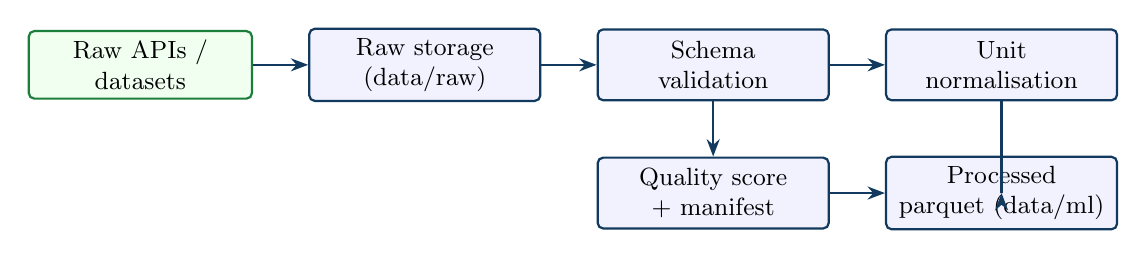
\begin{tikzpicture}[node distance=0.7cm and 0.7cm]
\node[src] (a) {Raw APIs /\\datasets};
\node[box, right=of a] (b) {Raw storage\\(data/raw)};
\node[box, right=of b] (c) {Schema\\validation};
\node[box, right=of c] (d) {Unit\\normalisation};
\node[box, below=of c] (e) {Quality score\\+ manifest};
\node[box, right=of e] (f) {Processed\\parquet (data/ml)};
\draw[flow] (a)--(b); \draw[flow] (b)--(c); \draw[flow] (c)--(d);
\draw[flow] (d)|-(f); \draw[flow] (c)--(e); \draw[flow] (e)--(f);
\end{tikzpicture}
\caption{Data ingestion and validation workflow (Figure 2).}
\label{fig:ingest}
\end{figure}

\begin{figure}[H]
\centering
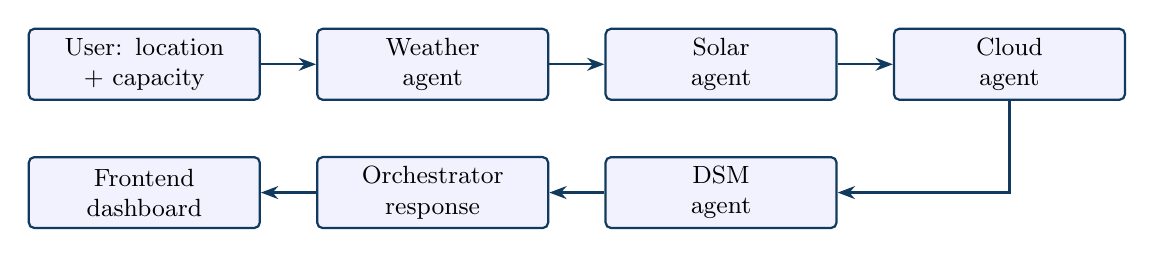
\begin{tikzpicture}[node distance=0.5cm and 0.7cm]
\node[box] (u) {User: location\\+ capacity};
\node[box, right=of u] (w) {Weather\\agent};
\node[box, right=of w] (s) {Solar\\agent};
\node[box, right=of s] (c) {Cloud\\agent};
\node[box, below=0.7cm of s] (d) {DSM\\agent};
\node[box, left=of d] (o) {Orchestrator\\response};
\node[box, left=of o] (fe) {Frontend\\dashboard};
\draw[flow] (u)--(w); \draw[flow] (w)--(s); \draw[flow] (s)--(c);
\draw[flow] (c)|-(d); \draw[flow] (d)--(o); \draw[flow] (o)--(fe);
\end{tikzpicture}
\caption{Forecast / orchestration workflow (Figure 3).}
\label{fig:orch}
\end{figure}

\begin{figure}[H]
\centering
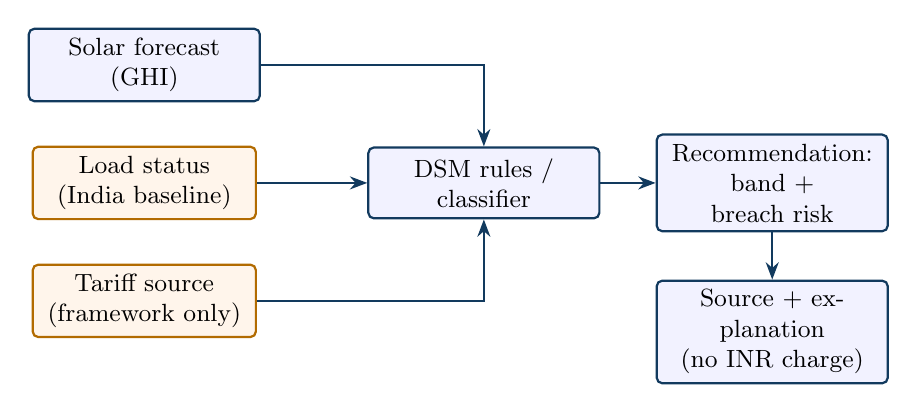
\begin{tikzpicture}[node distance=0.55cm and 0.7cm]
\node[box] (sf) {Solar forecast\\(GHI)};
\node[warn, below=of sf] (ld) {Load status\\(India baseline)};
\node[warn, below=of ld] (tf) {Tariff source\\(framework only)};
\node[box, right=1.4cm of ld] (m) {DSM rules /\\classifier};
\node[box, right=of m] (rec) {Recommendation:\\band + breach risk};
\node[box, below=0.6cm of rec] (ex) {Source + explanation\\(no INR charge)};
\draw[flow] (sf)-|(m); \draw[flow] (ld)--(m); \draw[flow] (tf)-|(m);
\draw[flow] (m)--(rec); \draw[flow] (rec)--(ex);
\end{tikzpicture}
\caption{DSM decision workflow (Figure 4). Orange nodes denote inputs that are
non-local or framework-only, so the output is a band/risk recommendation, not a rupee
settlement.}
\label{fig:dsm}
\end{figure}

% ================================================================== %
\section{API Layer}
The application registers 54 endpoints under \code{/api/v1} across 15 routers (introspected
from the FastAPI \code{app.routes} object). Table~\ref{tab:api} lists them. The Phase~1.7
\code{/agents/*} endpoints return a full provenance envelope
(\code{prediction\_type, model\_file, model\_version, training\_geography,
target\_geography, local\_data\_used, source\_status, confidence\_components,
production\_ready, data\_mode}).

\begin{footnotesize}
\begin{longtable}{@{}l p{6.2cm} l@{}}
\caption{Registered API endpoints (Table 6).}\label{tab:api}\\
\toprule
\textbf{Method} & \textbf{Path (/api/v1)} & \textbf{Provenance?}\\
\midrule
\endfirsthead
\toprule
\textbf{Method} & \textbf{Path} & \textbf{Provenance?}\\
\midrule
\endhead
\bottomrule
\endfoot
GET  & /health & --\\
GET  & /system/status & --\\
POST & /agents/solar/forecast & \yes\\
POST & /agents/cloud/risk & \yes\\
POST & /agents/dsm/assess & \yes\\
GET  & /agents/status & \yes\\
GET  & /agents/data-status & \yes\\
GET  & /sources ; /sources/\{id\} & \yes\\
GET  & /data-sources/status & \yes\\
POST & /dsm/check ; /dsm/advanced-check & partial\\
GET/POST & /dsm/rule-profiles ; /dsm/rule-profiles/\{id\} & \yes\\
POST & /dsm/karnataka/\{site\_id\} & partial\\
GET  & /locations ; /locations/available & --\\
GET  & /substations ; /substations/nearest/\{site\_id\} & \yes\\
POST & /substations/import & --\\
GET  & /weather/\{site\_id\} ; /weather/current/\{site\_id\} & \yes\\
GET  & /weather/latest/\{site\_id\} ; /weather/forecast/\{site\_id\} & \yes\\
POST & /weather/fetch ; GET /weather/providers/status & \yes\\
GET  & /forecast/\{site\_id\} & \yes\\
POST & /predict ; GET /predict/\{site\_id\} & \yes\\
GET  & /summary/\{site\_id\} ; /timeline/\{site\_id\} & partial\\
POST & /ml/train ; /ml/predict & \yes\\
POST & /ml/datasets/ingest-kaggle ; /ml/datasets/build-augmented & --\\
GET  & /ml/model/status & \yes\\
GET/POST & /sites ; /sites/\{id\} ; /sites/\{id\}/data-coverage & --\\
GET  & /energy/\{site\_id\} & partial\\
POST & /settle ; /settle/day/\{site\_id\} ; GET /settlements/\{site\_id\} & partial\\
GET/POST & /rl/rates ; /rl/runs ; /rl/train & partial\\
POST & /ingest/current/\{site\_id\} & --\\
GET  & /karnataka/regions ; /bescom/status ; POST /karnataka/seed & partial\\
GET  & /consumption/profiles & --\\
\bottomrule
\end{longtable}
\end{footnotesize}

% ================================================================== %
\section{Frontend Implementation}
The frontend is Next.js 14 with 13 page routes and shared components. A production build
succeeds and static-exports 14 routes (including \code{/\_not-found}).
Table~\ref{tab:frontend} lists the pages.

\begin{footnotesize}
\begin{longtable}{@{}p{2.2cm}p{2.6cm}p{4.0cm}c c@{}}
\caption{Frontend pages (Table 7).}\label{tab:frontend}\\
\toprule
\textbf{Page} & \textbf{Path} & \textbf{Purpose} & \textbf{Size} & \textbf{Status}\\
\midrule
\endfirsthead
\toprule
\textbf{Page} & \textbf{Path} & \textbf{Purpose} & \textbf{Size} & \textbf{Status}\\
\midrule
\endhead
\bottomrule
\endfoot
Root & app/page.tsx & landing & 176 B & \stC\\
Dashboard & app/dashboard & forecast + provenance panel & 5.3 kB & \stC\\
Data sources & app/data-sources & source/registry status & 3.6 kB & \stC\\
DSM & app/dsm & DSM check UI & 4.3 kB & \stC\\
ML & app/ml & model/metrics view & 4.3 kB & \stC\\
Locations & app/locations & sites/substations & 4.1 kB & \stC\\
System & app/system & health/status & 3.6 kB & \stC\\
Karnataka & app/karnataka & regional view & 3.7 kB & \stC\\
Predictions & app/predictions & prediction view & 4.1 kB & \stC\\
Timeline & app/timeline & time-series & 2.2 kB & \stC\\
Energy & app/energy & energy balance & 7.8 kB & \stC\\
Settlement & app/settlement & settlement view & 3.7 kB & \stC\\
RL & app/rl & RL rates/runs & 4.4 kB & \stC\\
\bottomrule
\end{longtable}
\end{footnotesize}

\noindent Components include \code{ModelProvenancePanel.tsx} (renders backend data mode,
geography, production readiness, and honesty warnings) and \code{OfflineBanner.tsx} (shows
an explicit offline state instead of faking data). ``Status'' here means the page builds
and renders; live data depends on a running backend.

% ================================================================== %
\section{Testing and Verification}
Table~\ref{tab:tests} lists commands actually run for this report and their outcomes.

\begin{table}[H]
\centering
\caption{Test / verification results (Table 9).}
\label{tab:tests}
\footnotesize
\begin{tabular}{@{}p{4.6cm}p{3.0cm}p{5.0cm}@{}}
\toprule
\textbf{Command} & \textbf{Result} & \textbf{Notes}\\
\midrule
\code{python -m pytest tests/ -q} & \stV\ 93 passed & 1 benign warning (CPU-count)\\
\code{ruff check app tests} & \stV\ all passed & no lint errors\\
\code{ruff format --check app tests} & \stP & 10 files would reformat (style only)\\
\code{npm run build} (frontend) & \stV\ success & 14 routes static-exported\\
FastAPI route introspection & \stV & 54 endpoints enumerated\\
\code{docker --version} & \stV & Docker 29.6.1 installed\\
\code{docker compose version} & \stM & ``unknown command: docker compose''\\
\code{docker compose config} & \stNV & cannot run (subcommand unavailable)\\
\code{docker info} (daemon) & \stNV & daemon unreachable\\
Kaggle load ingestion & \stV & 11{,}664 rows downloaded/used\\
NASA POWER cross-check & \stV & $r=0.87$ (manifest)\\
\bottomrule
\end{tabular}
\end{table}

% ================================================================== %
\section{Docker and Deployment State}
\code{docker-compose.yml} defines four services with healthchecks and a named volume.
Docker Engine is installed (v29.6.1) but the \code{docker compose} subcommand is
unavailable in this environment and the daemon is unreachable, so the stack was
\textbf{not} built or run. Deployment status is therefore \stNV.

\begin{table}[H]
\centering
\caption{Docker services (Table 8).}
\label{tab:docker}
\footnotesize
\begin{tabular}{@{}l l p{3.6cm}p{2.8cm}c@{}}
\toprule
\textbf{Service} & \textbf{Port} & \textbf{Purpose} & \textbf{Config} & \textbf{Verified?}\\
\midrule
postgres & 5432 & PostgreSQL 16 database & compose + healthcheck & \no\\
redis & 6379 & Redis 7 cache & compose + healthcheck & \no\\
backend & 8000 & FastAPI (build ./backend) & Dockerfile + healthcheck & \no\\
frontend & 3000 & Next.js (build) & Dockerfile + healthcheck & \no\\
pgdata & --- & Postgres volume & named volume & \no\\
\bottomrule
\end{tabular}
\end{table}

\noindent Note: \code{.env.example} is present but was not read for this report (blocked
by the workspace secret-file access policy); environment variables are inferred from
\code{app/config.py} (e.g.\ \code{APP\_DATA\_MODE}, \code{DATABASE\_URL},
\code{REDIS\_URL}, \code{WEATHER\_PROVIDER}).

% ================================================================== %
\section{Current Limitations}
\begin{itemize}[leftmargin=1.4em,itemsep=2pt]
\item \textbf{No local PV generation data.} Models predict irradiance; PV output is an
explicit estimate from user capacity, never measured or directly predicted.
\item \textbf{No metered Karnataka load/injection.} The only real load series is India
national (Kaggle); the load model is marked not production-ready (domain shift HIGH).
``Actual injection'' remains a nowcast/estimate.
\item \textbf{Tariff/DSM rupee rates not parsed.} CERC/KERC frameworks are verified, but
exact rates are market-linked and unparsed; DSM output is framework-only
(\code{emits\_rupee\_values=false}).
\item \textbf{Substation capacity unavailable.} OSM provides locations and partial
voltage (41\%) but no capacity; substation-level DSM is not claimed.
\item \textbf{Non-local baselines.} India-national load and HI-SEAS remain pretraining/
baseline only, never production truth.
\item \textbf{Docker not run.} Compose subcommand unavailable and daemon unreachable here.
\item \textbf{NASA POWER not a live provider.} Reachable and used as a build cross-check;
runtime provider integration is pending.
\item \textbf{RL not production-ready.} No policy trained; requires real local load,
solar, and official tariff reward.
\item \textbf{Lint format drift.} \code{ruff check} passes; \code{ruff format --check}
would reformat 10 files (cosmetic).
\end{itemize}

% ================================================================== %
\section{What Should Be Added Next}
\begin{footnotesize}
\begin{longtable}{@{}c p{3.2cm}p{3.0cm}p{2.6cm}p{2.6cm}@{}}
\caption{Prioritised roadmap (Table 10).}\label{tab:roadmap}\\
\toprule
\textbf{P} & \textbf{Addition} & \textbf{Why} & \textbf{Source required} & \textbf{Risk}\\
\midrule
\endfirsthead
\toprule
\textbf{P} & \textbf{Addition} & \textbf{Why} & \textbf{Source required} & \textbf{Risk}\\
\midrule
\endhead
\bottomrule
\endfoot
1 & Karnataka SLDC / Grid India load ingestion & localise load; unblock DSM/RL & KPTCL-SLDC / Grid India & portal/PDF, no API\\
2 & Official KERC/BESCOM tariff + CERC DSM parser & real INR DSM charges & KERC/CERC orders & PDF parsing, litigated rates\\
3 & Local PV generation ingestion & real PV target, not estimate & plant/BESCOM feed & availability\\
4 & Substation capacity enrichment & substation-level DSM & KPTCL/BESCOM/CEA & scanned maps\\
5 & NASA POWER live provider & second runtime weather source & NASA POWER API & LST alignment\\
6 & Strict global APP\_DATA\_MODE enforcement & block synthetic in all routes & (code) & legacy path refactor\\
7 & Docker full-stack verification & deployment readiness & Docker Desktop & env-specific\\
8 & Retrain load model on local data & production-grade load & item 1 & depends on item 1\\
9 & RL environment (after 1,2,3) & dispatch optimisation & real load+tariff & only after data exists\\
10 & Unify 1.5 registry + 1.7 provenance & single source-of-truth & (code) & low\\
\end{longtable}
\end{footnotesize}

% ================================================================== %
\section{Conclusion}
SuryaGrid AI is an architecturally complete multi-agent platform with a verified backend
(54 endpoints, 93 passing tests), a building frontend (14 routes), and an executed
real-data ML pipeline for Bengaluru weather/solar, substations, and India-baseline load.
Three models are production-ready for their stated (irradiance/risk/deviation-band) tasks;
the load model and RL policy are honestly marked not production-ready. It is \emph{not}
full production-ready: local PV, metered local load, official tariff rupees, and Docker
validation are outstanding.

\begin{table}[H]
\centering
\caption{Readiness classification.}
\label{tab:readiness}
\footnotesize
\begin{tabular}{@{}l l p{7.2cm}@{}}
\toprule
\textbf{Dimension} & \textbf{Level} & \textbf{Basis}\\
\midrule
Architecture & \stC & agents + API + frontend + ML pipeline all wired and running\\
Data & \stP & real weather/solar + substations + India load; local PV/load/capacity missing\\
ML & \stP & solar/cloud/DSM prod-ready; load non-local; RL not trained\\
DSM & \stP & framework + classifier; official INR rates pending\\
Deployment & \stNV & compose/Dockerfiles present; not built/run here\\
Production & \stPend & blocked on local PV, local load, official tariff, Docker validation\\
\bottomrule
\end{tabular}
\end{table}

% ================================================================== %
\section*{Appendix A: Key command outputs}
\addcontentsline{toc}{section}{Appendix A: Key command outputs}
\begin{lstlisting}
$ python -m pytest tests/ -q
93 passed, 1 warning in ~14s

$ ruff check app tests
All checks passed!

$ npm run build   (frontend, Next.js 14)
14 routes prerendered as static content (/, /dashboard, ... /timeline)

$ docker --version
Docker version 29.6.1, build 8900f1d
$ docker compose version
docker: unknown command: docker compose        # compose plugin unavailable

Build manifest (backend/data/ml/dataset_build_manifest.json):
  weather_solar_history: 26304 rows, 2022-01-01..2024-12-31,
    NASA POWER cross-check r=0.8728 (1096 days), peak GHI 1044 W/m2
  substations: 344 (voltage 41%, capacity 0%)
  load_history: 11664 rows (REAL_INDIA)
  rl_environment_dataset: NOT_AVAILABLE
\end{lstlisting}

\section*{Appendix B: Generated artifacts}
\addcontentsline{toc}{section}{Appendix B: Generated artifacts}
\textbf{Datasets} (\code{backend/data/ml/}): bengaluru\_weather\_solar\_history,
bengaluru\_substations\_cleaned, bengaluru\_grid\_features, solar\_agent\_training,
cloud\_agent\_training, dsm\_agent\_training, karnataka\_or\_india\_load\_history,
load\_agent\_training (all .parquet); dataset\_build\_manifest.json;
tariff\_dsm\_rules\_official\_or\_pending.json.\\
\textbf{Models} (\code{backend/models/trained/}): solar\_forecast\_model.pkl,
cloud\_risk\_classifier.pkl, dsm\_classifier.pkl, load\_forecast\_model.pkl,
dsm\_rules\_engine.json. (\code{rl\_policy.zip} absent by design.)\\
\textbf{Cards} (\code{backend/models/metadata/}): five \code{*\_card.json} +
training\_run\_manifest.json.

\section*{Appendix C: Documentation inventory}
\label{sec:docs}
\addcontentsline{toc}{section}{Appendix C: Documentation inventory}
\textbf{Present} (\code{docs/}): AGENT\_ARCHITECTURE, AGENT\_WORKFLOWS, API\_DESIGN,
API\_REFERENCE, BENGALURU\_DATA\_AND\_ML\_PIPELINE, BENGALURU\_DATA\_SOURCE\_RESEARCH,
BROWSER\_AND\_DATA\_ACCESS\_TEST, DATA\_SOURCE\_CATALOG, DEPLOYMENT, DOCKER\_ARCHITECTURE,
DSM\_RULE\_SOURCES, FINAL\_TOOL\_READINESS\_CHECK, FORMULA\_SOURCES,
LOCATION\_AND\_SUBSTATION\_DATA, ML\_PIPELINE, PHASE1\_SYSTEM\_VALIDATION,
REAL\_DATA\_PHASE1\_5, REAL\_DATA\_PHASE1\_7\_BENGALURU\_ML, SECURITY\_PLAN,
SOURCE\_REGISTRY, TOOLING\_AND\_BROWSER\_SETUP\_REPORT, formulas, and
substation\_data\_quality\_report, tariff\_and\_dsm\_source\_verification.\\
\textbf{Not present in repository:} \code{docs/REAL\_DATA\_PHASE1\_6.md},
\code{docs/limitations.md}. (Phase 1.6 was skipped; the project moved from 1.5 to 1.7.)

\vspace{1em}
\noindent\rule{\linewidth}{0.4pt}\\
{\footnotesize This report reflects the repository at commit state of 6 July 2026. Metrics
are quoted from model cards and manifests; endpoints from the live route table; test,
lint, and build results from the commands in Table~\ref{tab:tests}. Unverified items are
marked accordingly and not asserted as complete.}

\nocite{*}
\bibliographystyle{plain}
\bibliography{references}
\addcontentsline{toc}{section}{References}

\end{document}
